\documentclass[tikz,border=10pt]{standalone}

\usepackage{tikz}
\usetikzlibrary{arrows.meta, positioning, shapes.geometric,calc}

\begin{document}

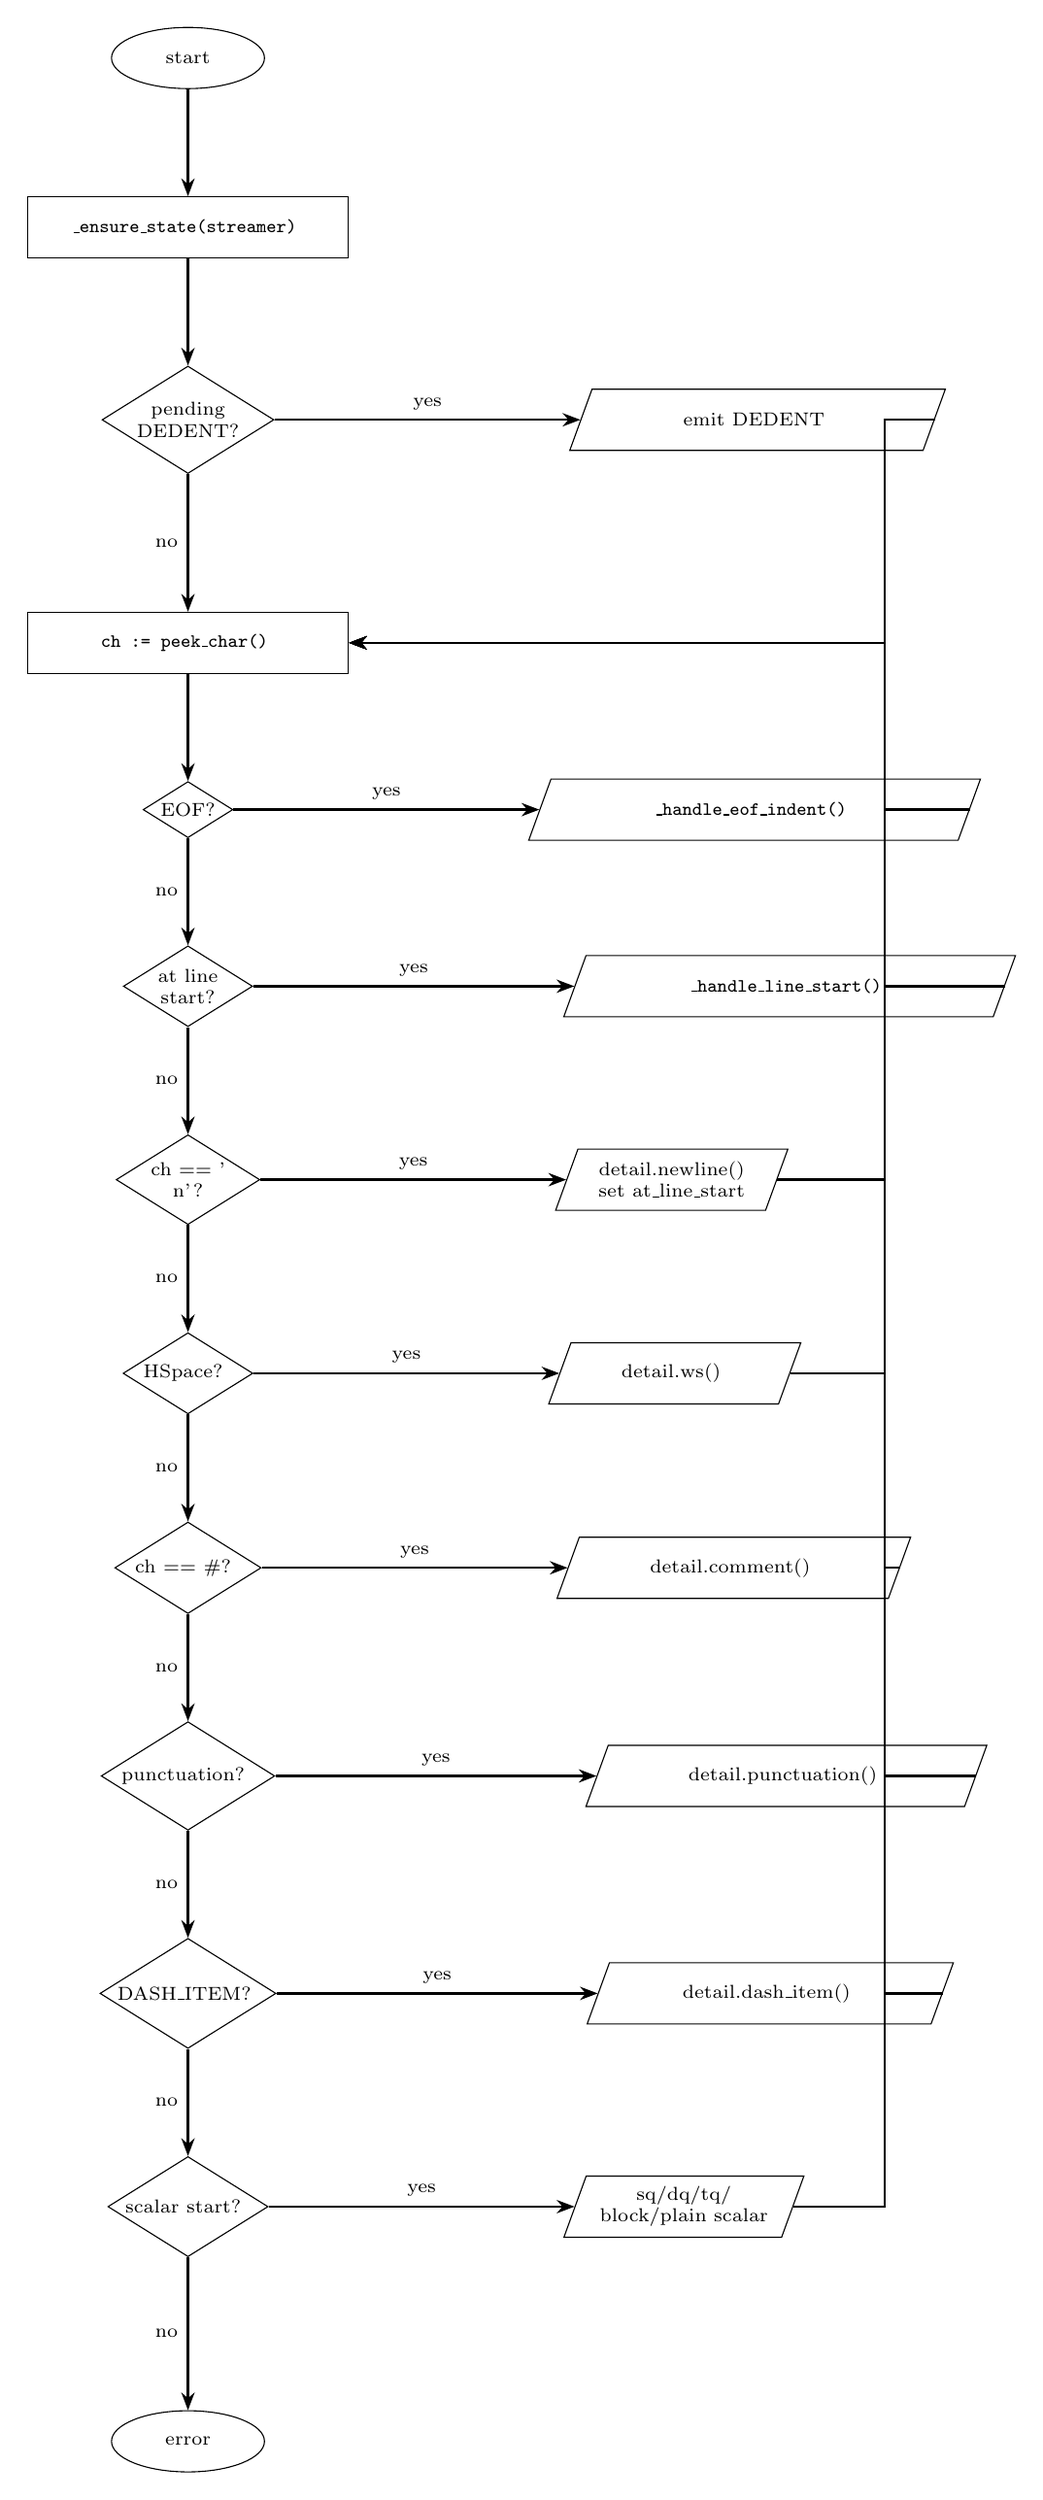
\begin{tikzpicture}[
  >=Stealth,
  node distance=1.4cm and 2.7cm,
  every node/.style={font=\scriptsize},
  startstop/.style={
    ellipse,
    draw,
    align=center,
    minimum width=2.0cm,
    minimum height=0.8cm
  },
  process/.style={
    rectangle,
    draw,
    align=center,
    minimum width=4.2cm,
    minimum height=0.8cm
  },
  decision/.style={
    diamond,
    draw,
    aspect=1.6,
    align=center,
    inner sep=1pt
  },
  io/.style={
    trapezium,
    trapezium left angle=70,
    trapezium right angle=110,
    draw,
    align=center,
    minimum width=3.0cm,
    minimum height=0.8cm
  },
  line/.style={->, thick}
]

% -------------------------------------------------------------------
% Main vertical flow
% -------------------------------------------------------------------
\node[startstop] (start) {start};

\node[process, below=of start] (ensure) {%
  \texttt{\_ensure\_state(streamer)}
};

\node[decision, below=of ensure] (pending) {%
  pending\\DEDENT?
};

\node[process, below=1.8cm of pending] (peek) {%
  \texttt{ch := peek\_char()}
};

\node[decision, below=of peek] (eof) {EOF?};

\node[decision, below=of eof] (atline) {%
  at line\\start?
};

\node[decision, below=of atline] (newline) {%
  ch == '\\n'?
};

\node[decision, below=of newline] (hspace) {%
  HSpace?
};

\node[decision, below=of hspace] (comment) {%
  ch == \#?
};

\node[decision, below=of comment] (punct) {%
  punctuation?
};

\node[decision, below=of punct] (dash) {%
  DASH\_ITEM?
};

\node[decision, below=of dash] (scalar) {%
  scalar start?
};

\node[startstop, below=2.0cm of scalar] (error) {error};

% -------------------------------------------------------------------
% Right-hand "emit & return" actions
% -------------------------------------------------------------------
\node[io, right=4.0cm of pending] (emitdedent) {%
  emit DEDENT
};

\node[io, right=4.0cm of eof] (eofindent) {%
  \texttt{\_handle\_eof\_indent()}
};

\node[io, right=4.2cm of atline] (linestart) {%
  \texttt{\_handle\_line\_start()}
};

\node[io, right=4.0cm of newline] (emitnewline) {%
  detail.newline()\\set at\_line\_start
};

\node[io, right=4.0cm of hspace] (emitws) {%
  detail.ws()
};

\node[io, right=4.0cm of comment] (emitcomment) {%
  detail.comment()
};

\node[io, right=4.2cm of punct] (emitpunct) {%
  detail.punctuation()
};

\node[io, right=4.2cm of dash] (emitdash) {%
  detail.dash\_item()
};

\node[io, right=4.0cm of scalar] (emitscalar) {%
  sq/dq/tq/\\block/plain scalar
};

% -------------------------------------------------------------------
% Main down arrows
% -------------------------------------------------------------------
\draw[line] (start) -- (ensure);
\draw[line] (ensure) -- (pending);
\draw[line] (pending) -- node[left]{no} (peek);
\draw[line] (peek) -- (eof);
\draw[line] (eof) -- node[left]{no} (atline);
\draw[line] (atline) -- node[left]{no} (newline);
\draw[line] (newline) -- node[left]{no} (hspace);
\draw[line] (hspace) -- node[left]{no} (comment);
\draw[line] (comment) -- node[left]{no} (punct);
\draw[line] (punct) -- node[left]{no} (dash);
\draw[line] (dash) -- node[left]{no} (scalar);
\draw[line] (scalar) -- node[left]{no} (error);

% -------------------------------------------------------------------
% Common "loop spine" to the far right
% -------------------------------------------------------------------
% A vertical spine to route all return arrows back to peek_char
\coordinate (spineBase) at ($(peek.east) + (7,0)$);
% helper coordinates for each emitting node projected onto spine x
\coordinate (spine_pending)   at (spineBase |- emitdedent.east);
\coordinate (spine_eof)       at (spineBase |- eofindent.east);
\coordinate (spine_atline)    at (spineBase |- linestart.east);
\coordinate (spine_newline)   at (spineBase |- emitnewline.east);
\coordinate (spine_hspace)    at (spineBase |- emitws.east);
\coordinate (spine_comment)   at (spineBase |- emitcomment.east);
\coordinate (spine_punct)     at (spineBase |- emitpunct.east);
\coordinate (spine_dash)      at (spineBase |- emitdash.east);
\coordinate (spine_scalar)    at (spineBase |- emitscalar.east);
\coordinate (spine_peek)      at (spineBase |- peek.east);

% -------------------------------------------------------------------
% Branch to actions, then route back along spine to peek_char()
% -------------------------------------------------------------------

% pending -> emitdedent -> spine -> up/down -> peek
\draw[line] (pending.east) -- node[above]{yes} (emitdedent.west);
\draw[line] (emitdedent.east) -- (spine_pending) -- (spine_peek) -- (peek.east);

% eof -> eofindent -> spine -> peek
\draw[line] (eof.east) -- node[above]{yes} (eofindent.west);
\draw[line] (eofindent.east) -- (spine_eof) -- (spine_peek) -- (peek.east);

% atline -> linestart -> spine -> peek
\draw[line] (atline.east) -- node[above]{yes} (linestart.west);
\draw[line] (linestart.east) -- (spine_atline) -- (spine_peek) -- (peek.east);

% newline -> emitnewline -> spine -> peek
\draw[line] (newline.east) -- node[above]{yes} (emitnewline.west);
\draw[line] (emitnewline.east) -- (spine_newline) -- (spine_peek) -- (peek.east);

% hspace -> emitws -> spine -> peek
\draw[line] (hspace.east) -- node[above]{yes} (emitws.west);
\draw[line] (emitws.east) -- (spine_hspace) -- (spine_peek) -- (peek.east);

% comment -> emitcomment -> spine -> peek
\draw[line] (comment.east) -- node[above]{yes} (emitcomment.west);
\draw[line] (emitcomment.east) -- (spine_comment) -- (spine_peek) -- (peek.east);

% punct -> emitpunct -> spine -> peek
\draw[line] (punct.east) -- node[above]{yes} (emitpunct.west);
\draw[line] (emitpunct.east) -- (spine_punct) -- (spine_peek) -- (peek.east);

% dash -> emitdash -> spine -> peek
\draw[line] (dash.east) -- node[above]{yes} (emitdash.west);
\draw[line] (emitdash.east) -- (spine_dash) -- (spine_peek) -- (peek.east);

% scalar -> emitscalar -> spine -> peek
\draw[line] (scalar.east) -- node[above]{yes} (emitscalar.west);
\draw[line] (emitscalar.east) -- (spine_scalar) -- (spine_peek) -- (peek.east);

\end{tikzpicture}

\end{document}

